\section{Introduction}
\label{section:intro-reactors}

In 2013, the \emph{Reactive Manifesto} \cite{manifest} defined the core principles of so-called \emph{Reactive systems}.
They are software systems, which aim to be

\begin{quote}
more flexible, loosely-coupled and scalable. 
This makes them easier to develop and amenable to change. 
They are significantly more tolerant of failure and when failure does occur they meet it with elegance rather than disaster.\hfill \cite{manifest}
\end{quote}

\noindent The manifesto does not mandate hard and fast rules for reactive systems.
Hence, over the years a variety of systems with different trade-offs have been created.\footnote{
    E.g. the cross-platform framework \emph{ReactiveX} and Apple's main UI-framework \emph{SwiftUI}.
}
Some of these systems are implicitly defined by their software implementations, while others define their behavior upon mathematical foundations.
In this thesis, we consider a specific model of computation for reactive systems called \emph{Reactors}.\footnote{
    An implementation of this model is realized by \emph{Lingua Franca} \cite{lf}.
}
The Reactor model aims at minimizing one of the downsides of reactive systems:

\begin{quote}
While scalability, resilience, elasticity, and responsiveness --- all tenets of the manifesto --- are clearly important, the gains in these dimensions come at the loss of testability due to the admittance of nondeterminism.
[...] We argue that the goals of reactive programming can also be achieved without adopting a nondeterministic programming model.\hfill \cite{cyphy}
\end{quote}

\noindent Loosely speaking, a system is considered \emph{deterministic} if multiple executions of the system on the same inputs exhibit the same behavior.
While determinism is rather common in closed software systems, it can be hard to maintain upon interaction with real-world components, like sensors, actuators, etc.
This is especially unfortunate in that these so-called \emph{cyber-physical systems} can come with a much higher cost of failure than purely digital systems.\footnote{
    For an example, cf. \cite{cyphy} Section 1.1.
}
A vital means for avoiding software failure, especially for larger systems, is traditional testing.
While software testability is determined by many factors, it is significantly impaired if the system under test is inherently nondeterministic \cite[p.~7]{marten}. 
Hence, the Reactor model's stride towards \emph{determinism} is also a stride towards \emph{testability}.\footnote{
    For a complete discussion of the benefits of Reactors, cf. \cite{cyphy} and \cite{marten}.
}

While the Reactor model aims at being deterministic under certain conditions, its determinism is yet unproven.
Proving this claim is also hindered by the fact that the model lacks a well-defined formalization.
Thus, the first goal of this thesis is to provide a well-defined subset of the model.

\break

\subsection{Reactor Model}

In this section we start by giving a very brief overview of Reactors.
Further details are discussed in subsequent sections.

\begin{figure}[h]
\centering
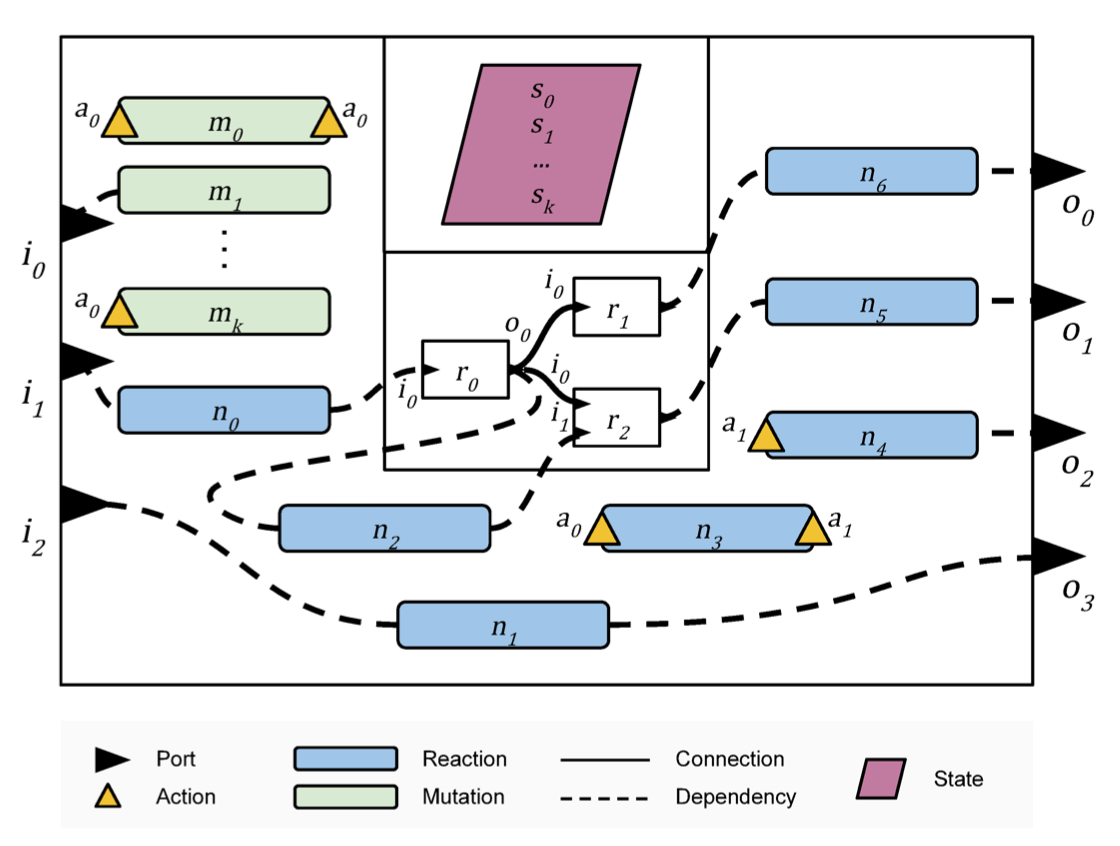
\includegraphics[width=0.8\columnwidth]{reactor}
\caption{Schematic representation of a reactor \cite{cyphy}}
\label{fig:reactor}
\end{figure}

\paragraph{Components:}

The Reactor model is best understood visually --- Figure \ref{fig:reactor} illustrates most of its components. 
The entirety of the illustration shows a single \emph{reactor}, which serves as an isolated container of functionality. 
Communication, i.e. data flow, between different reactors is achieved by their \emph{ports}. 
Ports can be written to and read from, and therefore carry \emph{values}.
The main components that read and write values are called \emph{reactions}. 
They can be considered the atomic functional units within a reactor. 
Reactions are \emph{triggered} by incoming values, perform computations on those values and produce a resulting output. 
Aside from their purely functional aspect though, reactions also have access to mutable \emph{state} that is shared among all reactions in a given reactor.

The full Reactor model has a breadth of additional components and features that allow modeling complex behaviors \cite[pp.~18-40]{marten}.
For the sake of brevity, this thesis will only consider a subset of those features, which we call the \emph{Simple Reactor} model.

\paragraph{Semantic Time:}

The Simple Reactor model, as described so far, is purely instantaneous --- it has no notion of time. 
A key feature of the Reactor model, is its \emph{semantic notion of time}.
It introduces two distinct variants of time: \emph{logical} and \emph{physical}. 
While physical time represents ``real'' time, as on a clock, logical time is a system-internal notion.
That is, the separation between the digital and the physical worlds that is present in cyber-physical systems, is applied to time as well \cite[p.~235]{dense}.
Separating these two notions of time makes it possible to reason deterministically about events in logical time, while still allowing for interaction with physical time under explicitly defined semantics.
While the details of these interactions are not explored in this thesis, we will reap some of the benefits of logical time in later sections.
For example, we can easily define an order of execution of events within logical time, such that we need not care about their actual runtimes.
Adding a notion of physical time would further allow us to impose physical time limits on their execution.

\paragraph{Actions:}

Time manifests itself in reactors through \emph{actions}.
They provide a means for reactions to send and receive values \emph{over time}. 
The distinct notions of time described above carry over to distinct notions of actions --- there are physical and logical actions. 
A reaction can \emph{schedule} a logical action, to occur at a specific logical time in the future. 
When that time is reached, the target of that action will receive a specified value as input.
Physical actions on the other hand have external origins --- they are scheduled by entities like physical sensors.
In the Simple Reactor model, we only consider \emph{logical} time and its actions.

\subsection{Simple Reactor Model}
\label{section:simpel-reactors}

In this section we define the Simple Reactor model as a subset of the full Reactor model (with minor changes).
The definitions given here may change considerably in the rigorous formalization presented in Section \ref{section:formal-inst-reactors}, as they contain problematic inaccuracies.\footnote{Cf. Section \ref{section:inaccuracies}.}
Additionally, the following definitions may be partially redundant. 
This is a result of trying to remove any aspects not relevant to readers unfamiliar with \cite{cyphy}, while still showing how this model is obtained by reducing the full Reactor model.

\paragraph{Identifiers \& Values:}

Two of the primitive notions in the Reactor model are \emph{identifiers} and \emph{values}.
Identifiers, defined as members of a set $\Sigma$, are used to refer to a variety of components within the Reactor model: state variables, actions, ports, etc.
A set of values $\mathfrak{V}$ contains opaque values that are the ``data'' upon which computation takes place.
We require that $\mathfrak{V}$ contain a special value $\epsilon$ called the \emph{absent value}.
The opaque nature of identifiers and values shows that our model does not depend on their structure.\footnote{ 
  We will see in Section \ref{section:time-primitives} that it \emph{can} be useful to add some well-defined structure to them.
}

\paragraph{Tags:} 

Logical time progresses in discrete steps. 
For each of those steps we define a \emph{tag}, as an element of $\mathbb{T} = \mathbb{N} \times \mathbb{N}$.
For a tag $t = (v, m)$ we call $v$ the \emph{time value} and $m$ the \emph{microstep index}.
Notationally, we reference fields of a tuple by their given names. 
For example, for a given tag $t$, its time value can be referenced as $v(t)$ and its microstep index as $m(t)$.
This representation of time is called \emph{superdense} \cite{dense}, as it allows us to step through an arbitrary number of tags before reaching a new time value.
The order of these tags is given by their lexicographical order\footnote{
    For tags $t_1$ and $t_2$: $t_1 \leq t_2$ if $v(t_1) < v(t_2)$ or $v(t_1) = v(t_2)\ \wedge\ m(t_1) \leq m(t_2)$.
}.

\paragraph{Actions:} 

An action $a$ is defined as $a = (x, d, \mathfrak{o})$, where:

\begin{enumerate}
    \item $x \in \Sigma$ is the action's \emph{identifier}.
    \item $d \in \mathbb{N}$ is the \emph{delay} --- an offset from the current logical time that specifies when the action should be scheduled.
    \item $\mathfrak{o} \in \mathfrak{O}$ is the \emph{origin} --- a descriptor for whether the action is logical or physical.
    Since the Simple Reactor model only allows for logical actions, the set $\mathfrak{O}$ of \emph{origins} can be described by the unit set $\{logical\}$, and is therefore redundant.
\end{enumerate}

\noindent Scheduling an action implies the creation of an event.
The value carried by an action is placed in its corresponding event.

\paragraph{Events:} 

An event $e$ is defined as $e = (\mathfrak{t}, \mathfrak{v}, \mathfrak{g})$, where:

\begin{enumerate}
    \item $\mathfrak{t} \in \Sigma$ is the \emph{event trigger} --- the object that scheduled the event.
    \item $\mathfrak{v} \in \mathfrak{V}$ is the \emph{trigger value} --- the value to be associated with $\mathfrak{t}$ when the event occurs.
    \item $\mathfrak{g} \in \mathbb{T}$ is the \emph{event tag} --- the logical time at which the event should occur.
\end{enumerate}

\paragraph{Reactors:}

A reactor $rtr$ is defined as a tuple $rtr = (I, O, A, S, N, P)$, where:

\begin{itemize}
    \item $I \subseteq \Sigma$ is the set of \emph{input ports}.
    \item $O \subseteq \Sigma$ is the set of \emph{output ports}.
    \item $S \subseteq \Sigma$ is the set of \emph{state variables}.
    \item $A \subseteq \Sigma \times \mathbb{N} \times \mathfrak{O}$ is the set of \emph{actions}.
    \item $\mathcal{N}$ is the set of \emph{reactions}.
    \item $P: \mathcal{N} \to \mathbb{N}$ is the \emph{priority function} --- an injective map from reactions to their priorities.
    Priorities are used to determine order of execution for reactions.
    The full Reactor model does not require this function to be injective, thereby allowing multiple reactions to have the same priority.
    This is a deliberate choice, as it allows non-determinism to be introduced if explicitly chosen. 
    The Simple Reactor model requires reactions to have unique priorities, as this imposes a total order on them, which simplifies the proof of determinism.
\end{itemize}

\paragraph{Reactions:}

\noindent A reaction $rcn$ is defined as $rcn = (D, T, B, D^\vee, H)$. Let $\mathcal{C}$ be the reactor that contains $rcn$, then:

\begin{enumerate}
    \item $D \subseteq I(\mathcal{C})$ is the set of \emph{dependencies} --- ports that can be accessed when the reaction executes.
    \item $\mathcal{T} \subseteq D \cup x(A(\mathcal{C}))$ is the set of \emph{triggers} --- ports and actions that cause the execution of the reaction's body, when set to a non-absent value.
    \item $B$ is the \emph{body} of the reaction, which is opaque executable code.
    \item $D^\vee \subseteq O(\mathcal{C})$ is the set of \emph{antidependencies} --- ports that can be written to when the reaction executes.
    \item $H \subseteq x(A(\mathcal{C}))$ is the set of \emph{schedulable actions} --- actions for which the reaction can generate events.
\end{enumerate}

\paragraph{Reactor Networks:}

In the full Reactor model the mechanism for creating a \emph{network} of reactors is given by a reactor's ability to define \emph{nested reactors}. 
As we do not account for this feature in the Simple Reactor model, we need to define a separate mechanism for creating networks.
Hence, we define a reactor network $\sigma$ as a graph structure $\sigma = (R, E)$, where:

\begin{enumerate}
    \item $R$ is the set of \emph{reactors}.
    \item $E \subseteq \Sigma \times \Sigma$ are the directed \emph{edges} connecting reactors' ports.
\end{enumerate}

\subsubsection{Execution Model}
\label{section:exec-model}

The execution model as presented in \cite{cyphy} is defined by a given set of procedures.
Here we present the execution model \emph{visually} instead of \emph{algorithmically} for two reasons:

\begin{itemize}
    \item The procedures in \cite{cyphy} need to handle many features (like physical actions) which we have omitted in the Simple Reactor model.
    Any attempt at reducing the algorithms would retain no more than a vague correspondence. 
    \item An algorithm that uses the definitions stated above, would diverge greatly from the rigorous algorithms presented in Section \ref{section:formal-inst-reactors}, and thus have little utility.
\end{itemize}

\paragraph{Prerequisites:}

We define computation for reactor \emph{networks}.
Our definition is rudimentary in that we define no real starting point.
That is, we simply begin computation upon whatever state our given reactor network is in, without any previous setup.\footnote{
    This is in contrast to the full Reactor model, which defines initialization actions.
}
To perform computations, we require three additional objects:
\break

\begin{itemize}
    \item A global tag --- since we only consider logical time, this is our only time keeping mechanism.
    \item An event queue --- a list of events to be processed, ordered by their tags.
    As actions are scheduled, events are added to this queue.
    Execution is complete when this queue is empty.
    \item A precedence graph --- a graph that manifests the dependencies between reactions in the network.
    This is used to determine the order in which reactions should be executed.
\end{itemize}

\noindent Let Figure \ref{fig:reactor-network} illustrate our reactor network.
We have three reactors, $R1$, $R2$ and $R3$ with a total of five reactions.
$R1$ can propagate data from its output ports, to $R2$ and $R3$.
$R2$ can propagate data back to itself, as well as to $R3$.
The only reactor that uses actions is $R1$.

\begin{figure}[!h]
\centering
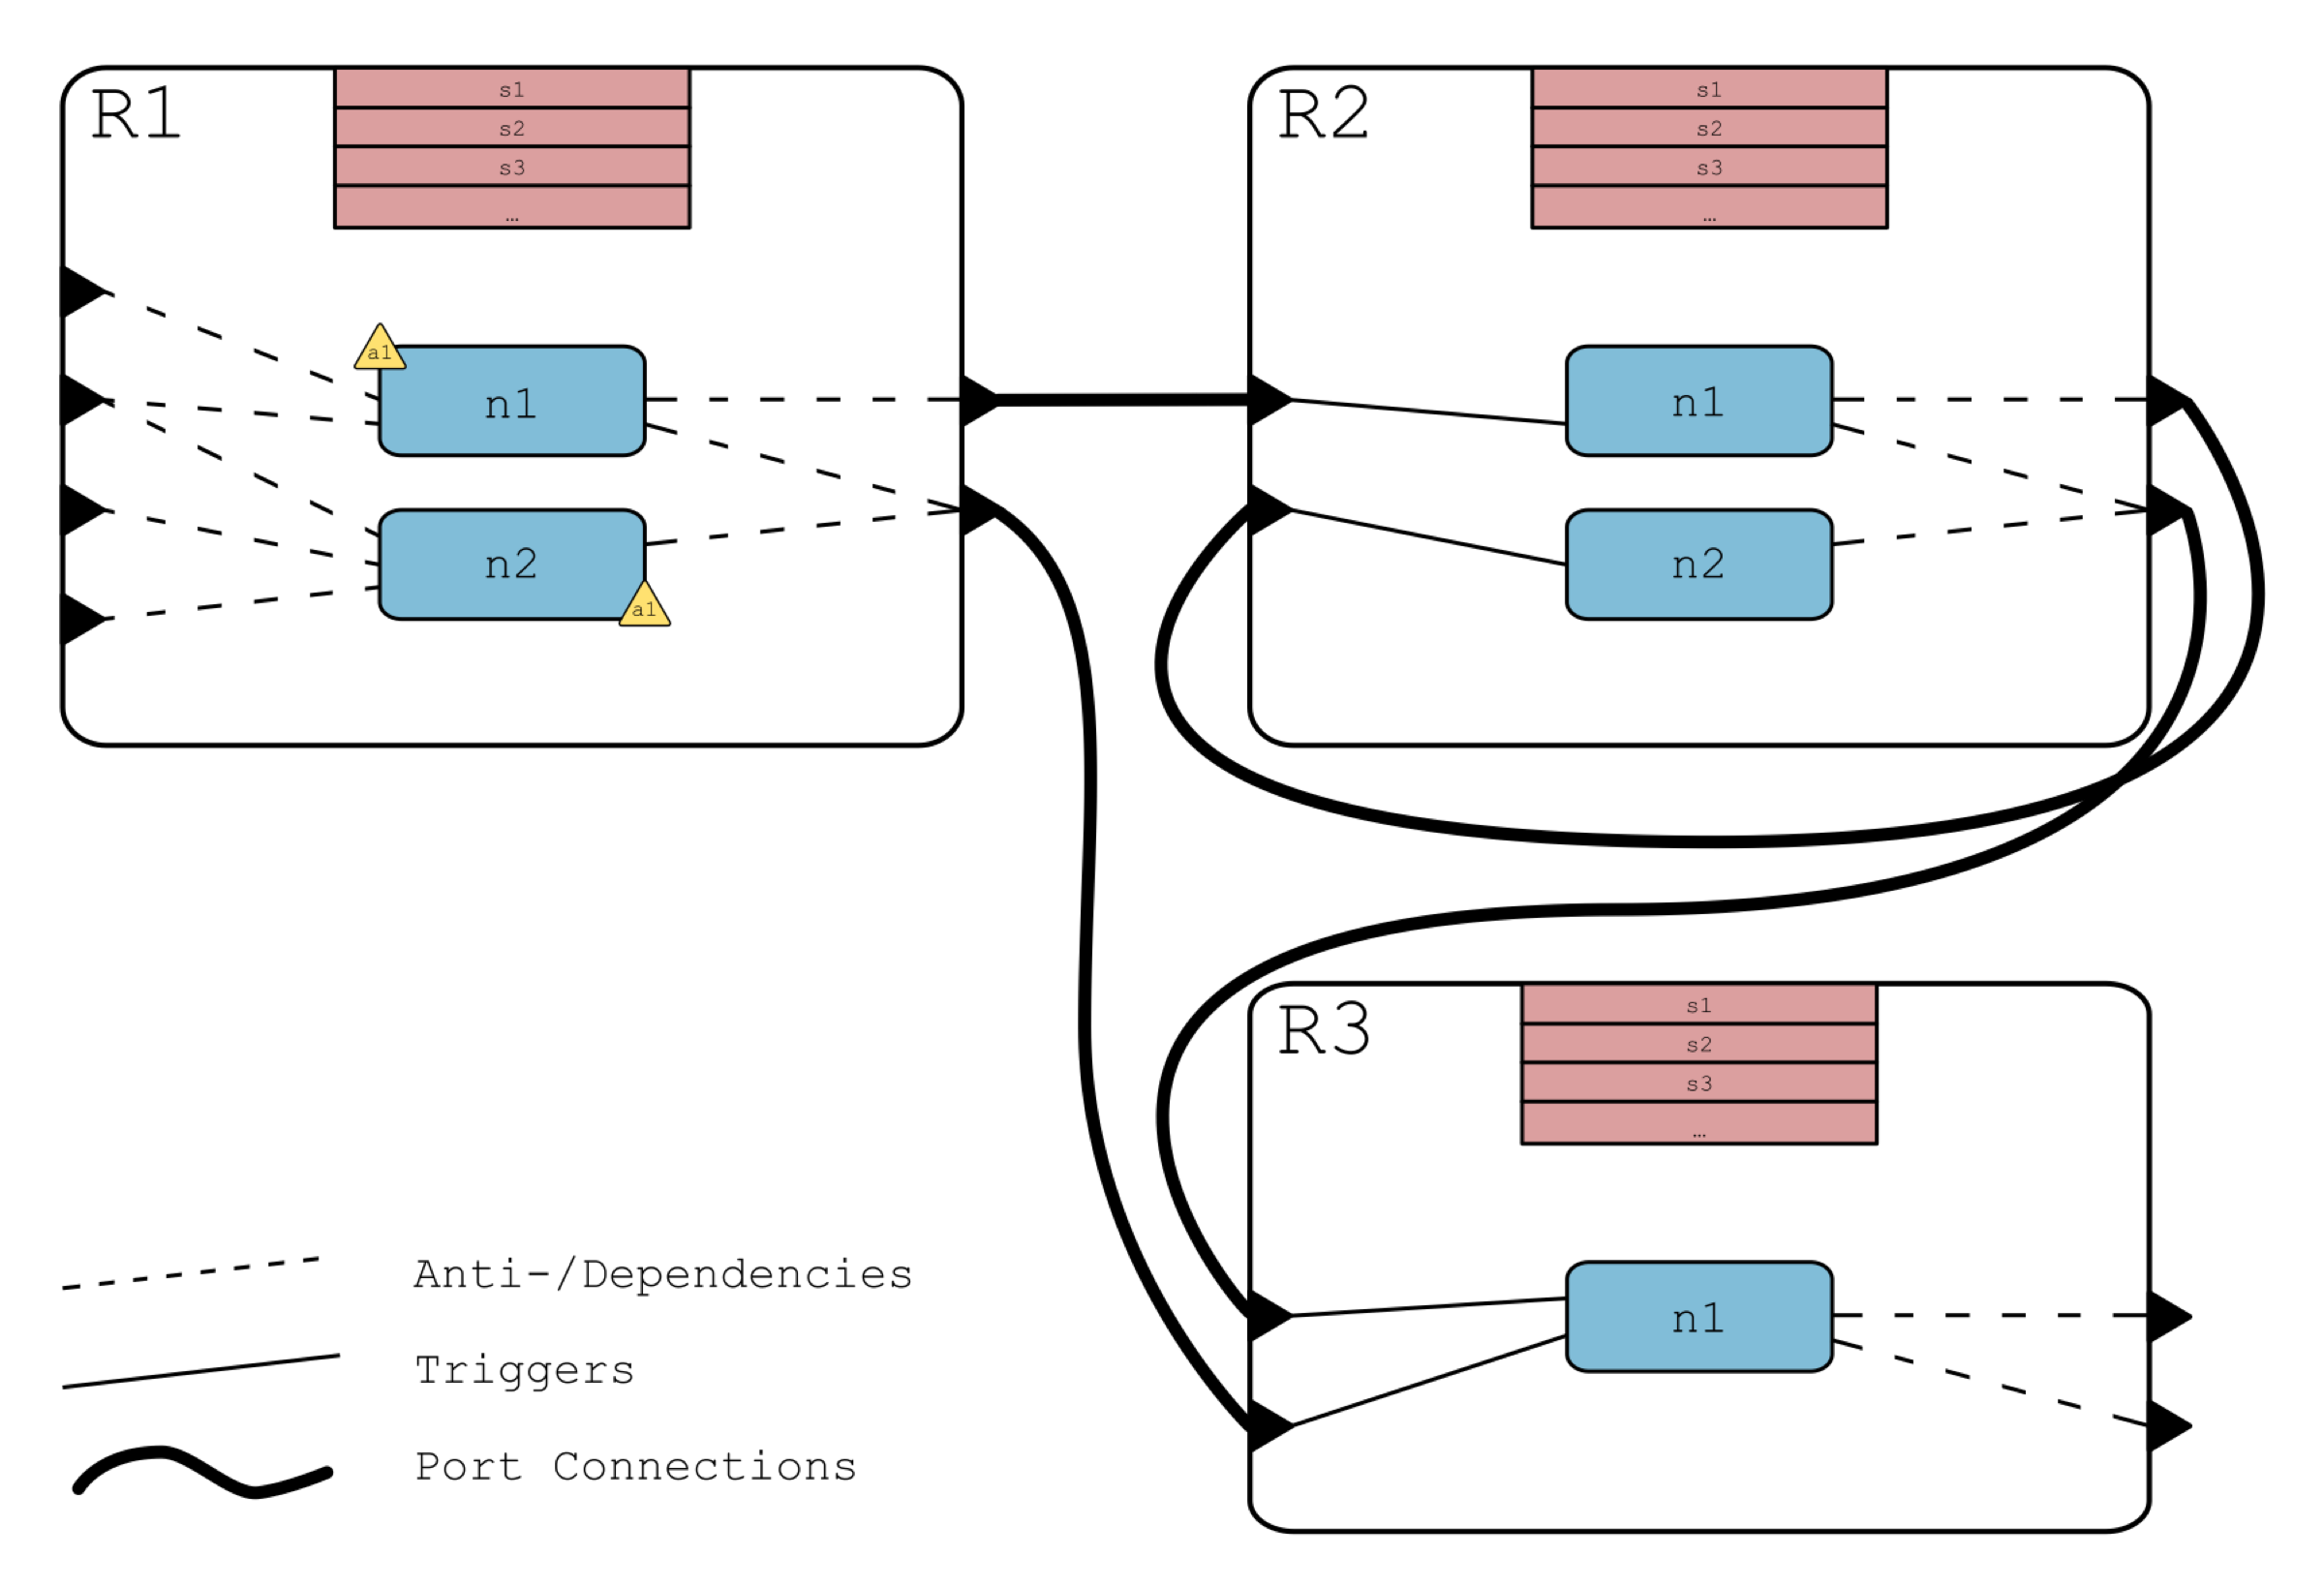
\includegraphics[width=0.95\columnwidth]{reactor-network}
\caption{Reactor network}
\label{fig:reactor-network}
\end{figure}

\noindent The precedence graph for this network is illustrated in Figure \ref{fig:precedence-graph}.\footnote{
    An algorithm for computing precedence graphs is presented in \cite{cyphy}.
}
We obtain this graph by placing edges between reactions according to their priorities within a reactor, as well as the connections between their anti/-dependencies.
Notably, our precedence graph contains no cycles.
This is an important restriction of the Reactor model: we only define computation for reactor networks that have acyclic precedence graphs.
Without this restriction, it wouldn't be possible to deterministically define an order of execution, as each reaction would depend on some other reaction before it could execute.
With an acyclic precedence graph, we define reactions' order of execution as a topological ordering over the precedence graph.\footnote{
    If it were not acyclic, such an ordering would not exist.
}
Thus, we don't require the precedence graph itself for execution, but rather a topological ordering ($\mathcal{Q}_R$) over it:

\vspace{2mm}
$\mathcal{Q}_R = [R1.n1,\ R1.n2,\ R2.n1,\ R2.n2,\ R3.n1]$
\vspace{2mm}

\begin{figure}[!h]
\centering
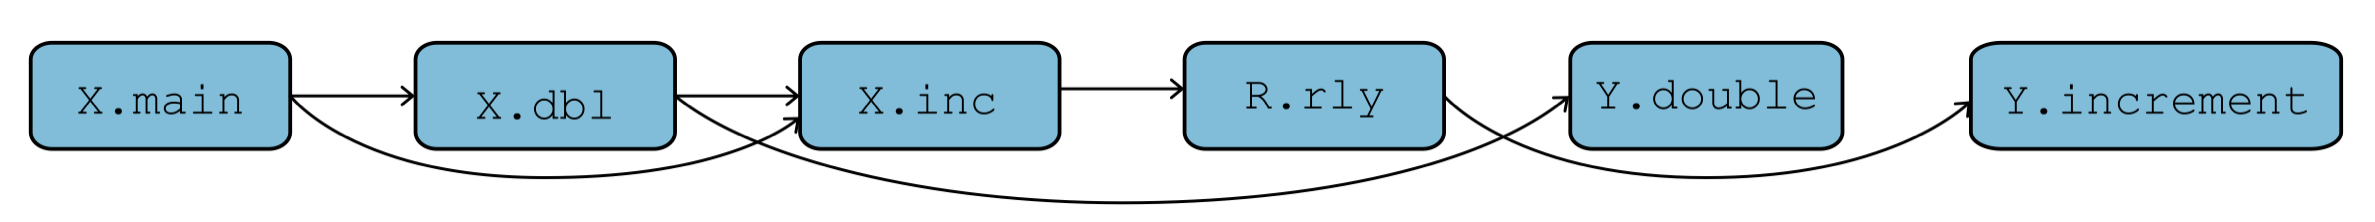
\includegraphics[width=\columnwidth]{precedence-graph}
\caption{Precedence graph}
\label{fig:precedence-graph}
\end{figure}

\paragraph{Execution:}
\label{section:execution-model-steps}

Using these prerequisites, we can describe how to execute a reactor network.

\begin{enumerate}
    \item Increase the global tag to match the next event $e$ in the event queue.
    If there is none, execution has completed.

    \item Run each reaction in the order defined by $\mathcal{Q}_R$:
    \begin{enumerate}
        \item Check if the reaction is triggered by its dependencies, i.e. if at least \emph{some} trigger is non-absent.
        \item If so, run the reaction's body. 
        If not, advance to the next reaction.
        \item For each action scheduled during the body's execution, add a corresponding event to the event queue.
        Actions can only be scheduled with a tag \emph{greater} than the current one.\footnote{
            An action's event's tag is a result of the \emph{delay} specified by the action. 
            If a delay of $0$ is specified, then a microstep delay of $1$ is added.
        }
        \item For each output port written to by the reaction's body, propagate the values to any connected ports.
    \end{enumerate}

    \item Clear all ports, dequeue all events for the current tag, and go to Step 1.
\end{enumerate}

\paragraph{Example:}

We can visualize these steps with an example. 
Let Figure \ref{fig:exec-0} be the initial state of our reactor network.
That is, our current tag is $(4,2)$, we have one event in the event queue and all ports are set to $\epsilon$.

\begin{itemize}[leftmargin=0pt]
    \item[] Figure \ref{fig:exec-1}: 
    Our first step is to increase the tag to $(5,0)$, as that's the tag of the next event.
    We then start executing the reactions with $R1.n1$.
    We assume here, that $a1$ belongs to its triggers and thus $R1.n1$ triggers.
    Thus, $R1.n1$'s body executes and aside from its port-dependencies (which are all $\epsilon$), it receives the value $V$ specified for $a1$ at the current tag. 
    \item[] Figure \ref{fig:exec-2}: 
    $R1.n1$ cannot schedule any actions (according to the illustration), but we assume here that $R1.n1$'s body produces outputs $W$ and $X$ for its ports respectively.
    After propagating those values to all connected ports we progress to the execution of reaction $R1.n2$. 
    \item[] Figure \ref{fig:exec-3}:
    $R1.n2$ does not trigger for the given state, so we progress to $R2.n1$ immediately.
    $R2.n1$'s trigger is non-absent, so we execute it, producing output values $Y$ and $Z$.
    \item[] Figure \ref{fig:exec-4}:
    $R2.n2$ triggers, as its trigger is non-absent.
    Assuming the reaction outputs some value $O$, this values overrides the current value $Z$ of its output port and is propagated to $R3$.
    \item[] Figure \ref{fig:exec-5}:
    Lastly, $R3.n1$ triggers, as at least one of its triggers (and in fact both) is non-absent.
    We assume here that it does produce any output during execution.
    Thus, we have run all reactions and progress to Step 3 of execution.
    Here we set all ports to $\epsilon$ again and remove all events with tag $(5,0)$ from the event queue. 
\end{itemize} 

\noindent The resulting event queue is empty and we have fully executed this network.

\begin{figure}[!htbp]
\centering
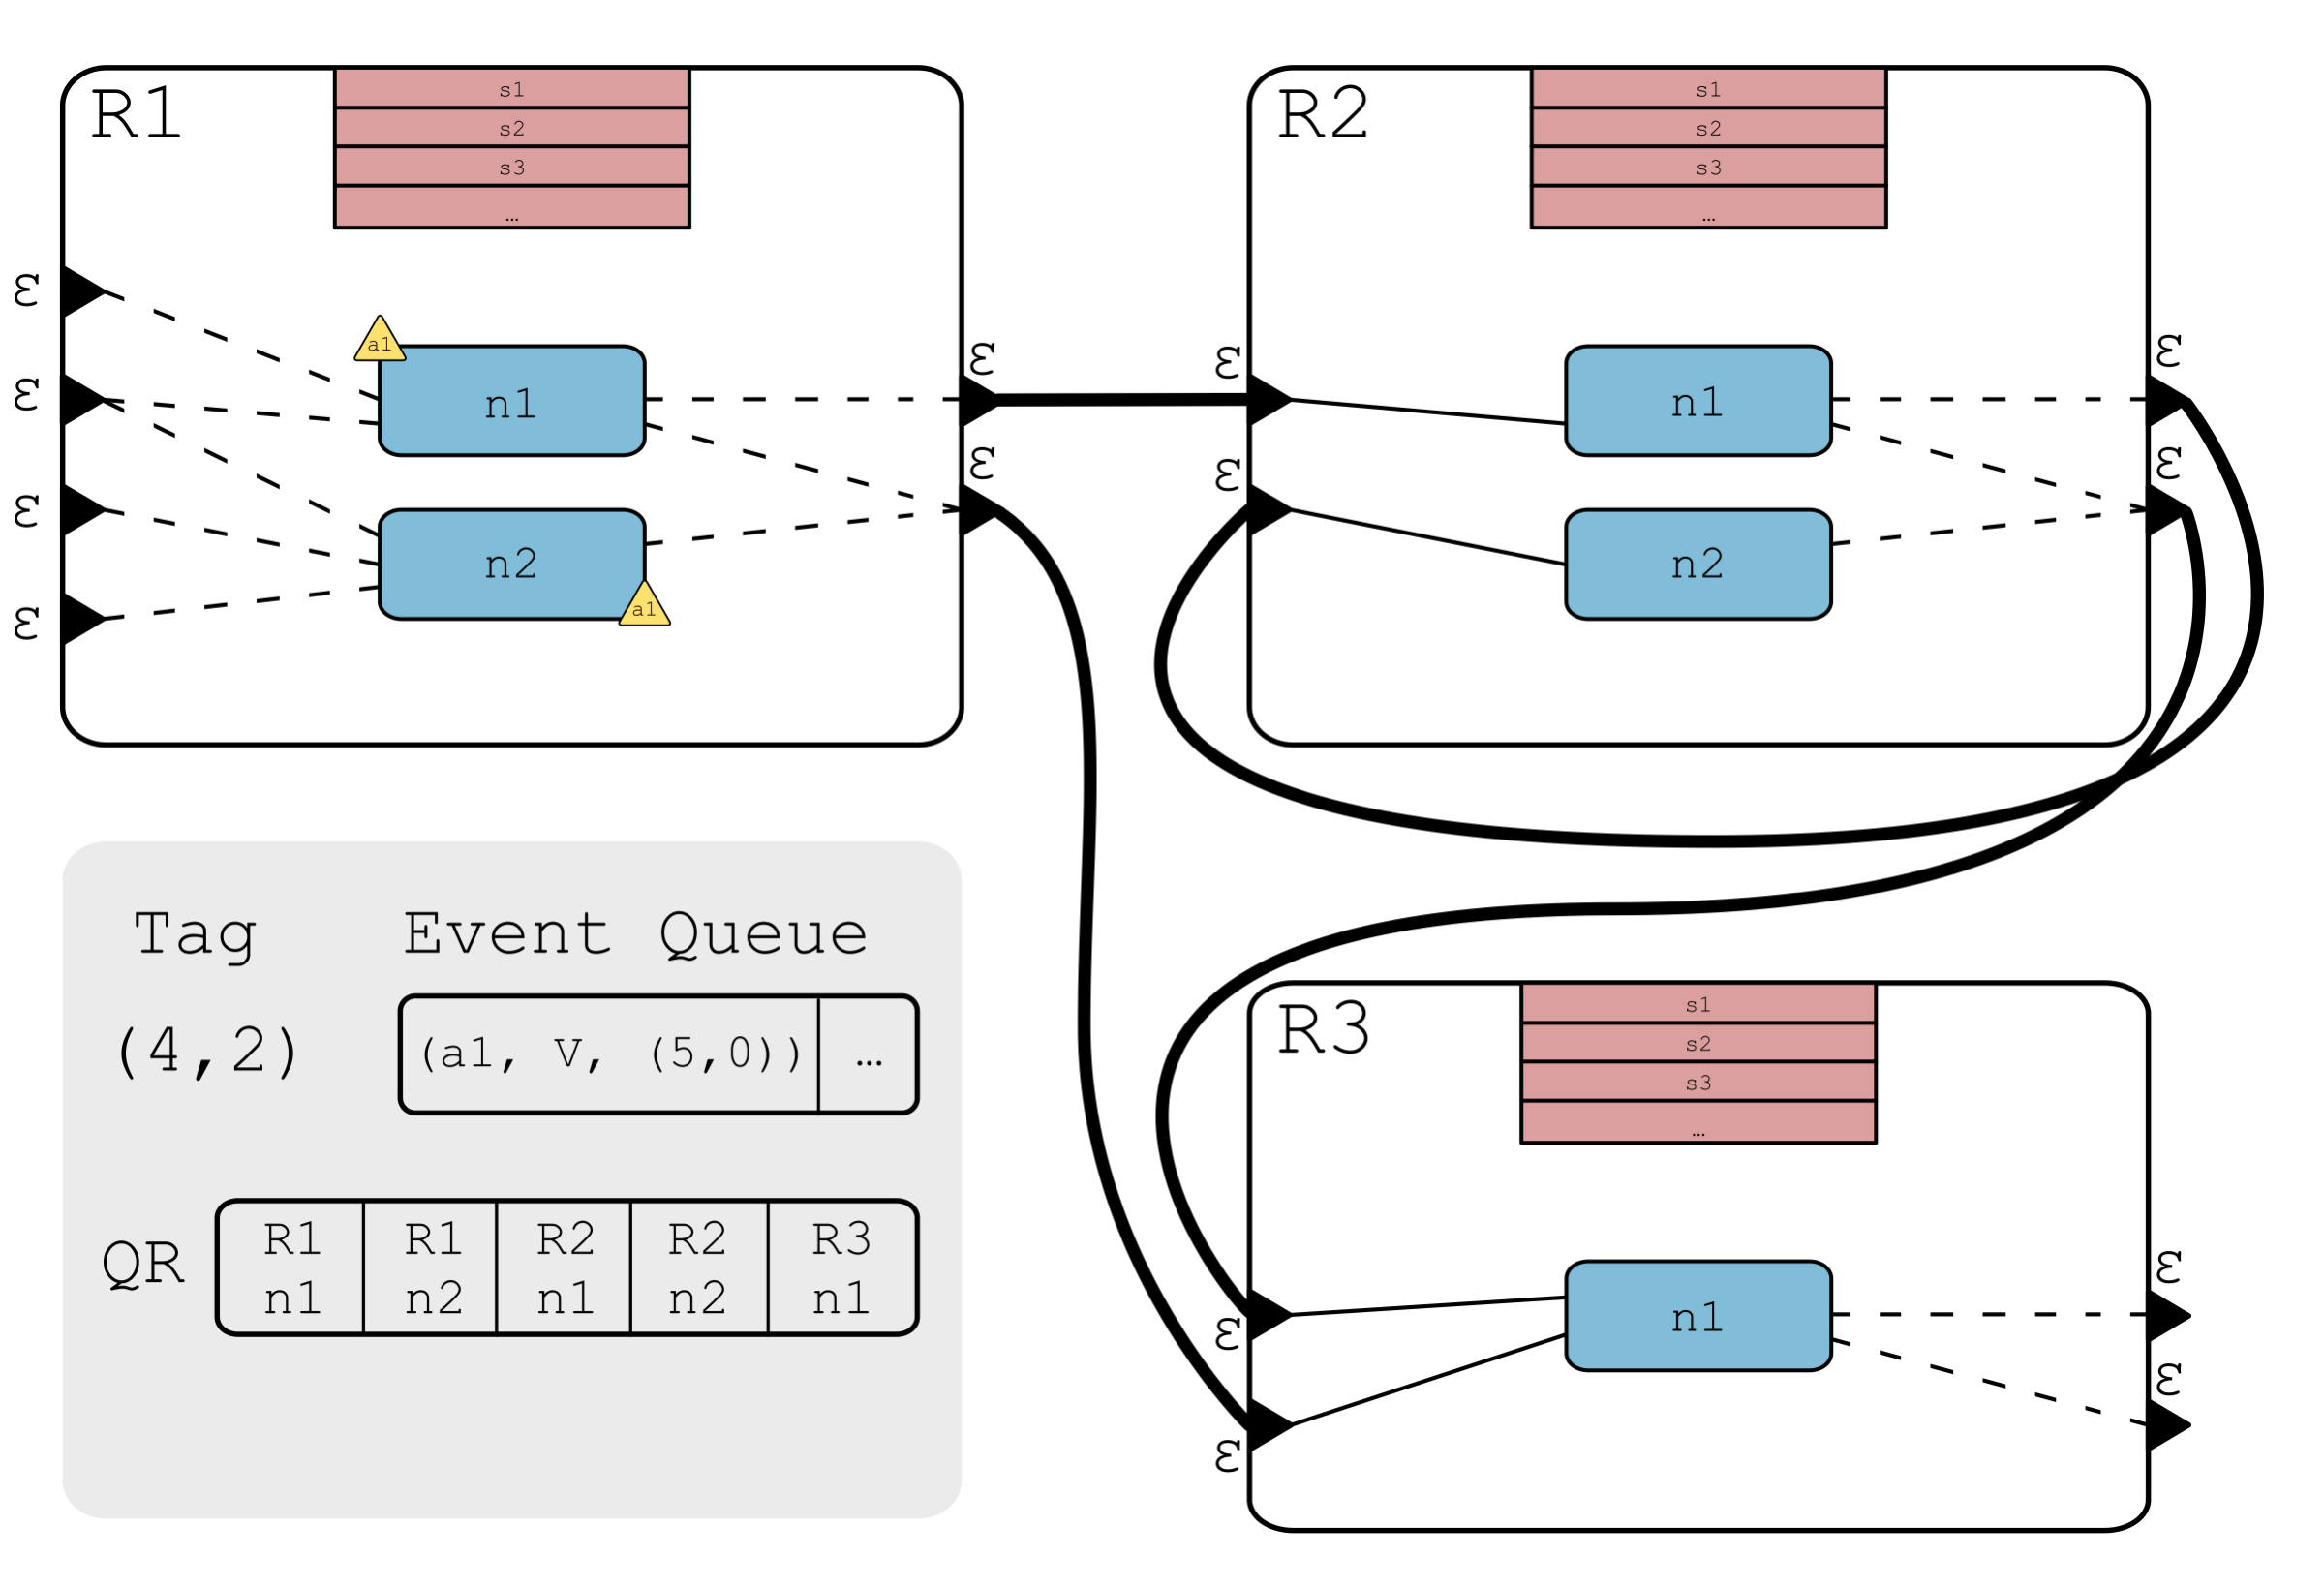
\includegraphics[width=\columnwidth]{exec-0}
\caption{Execution example --- initial state}
\label{fig:exec-0}
\end{figure}

\begin{figure}[!htbp]
\centering
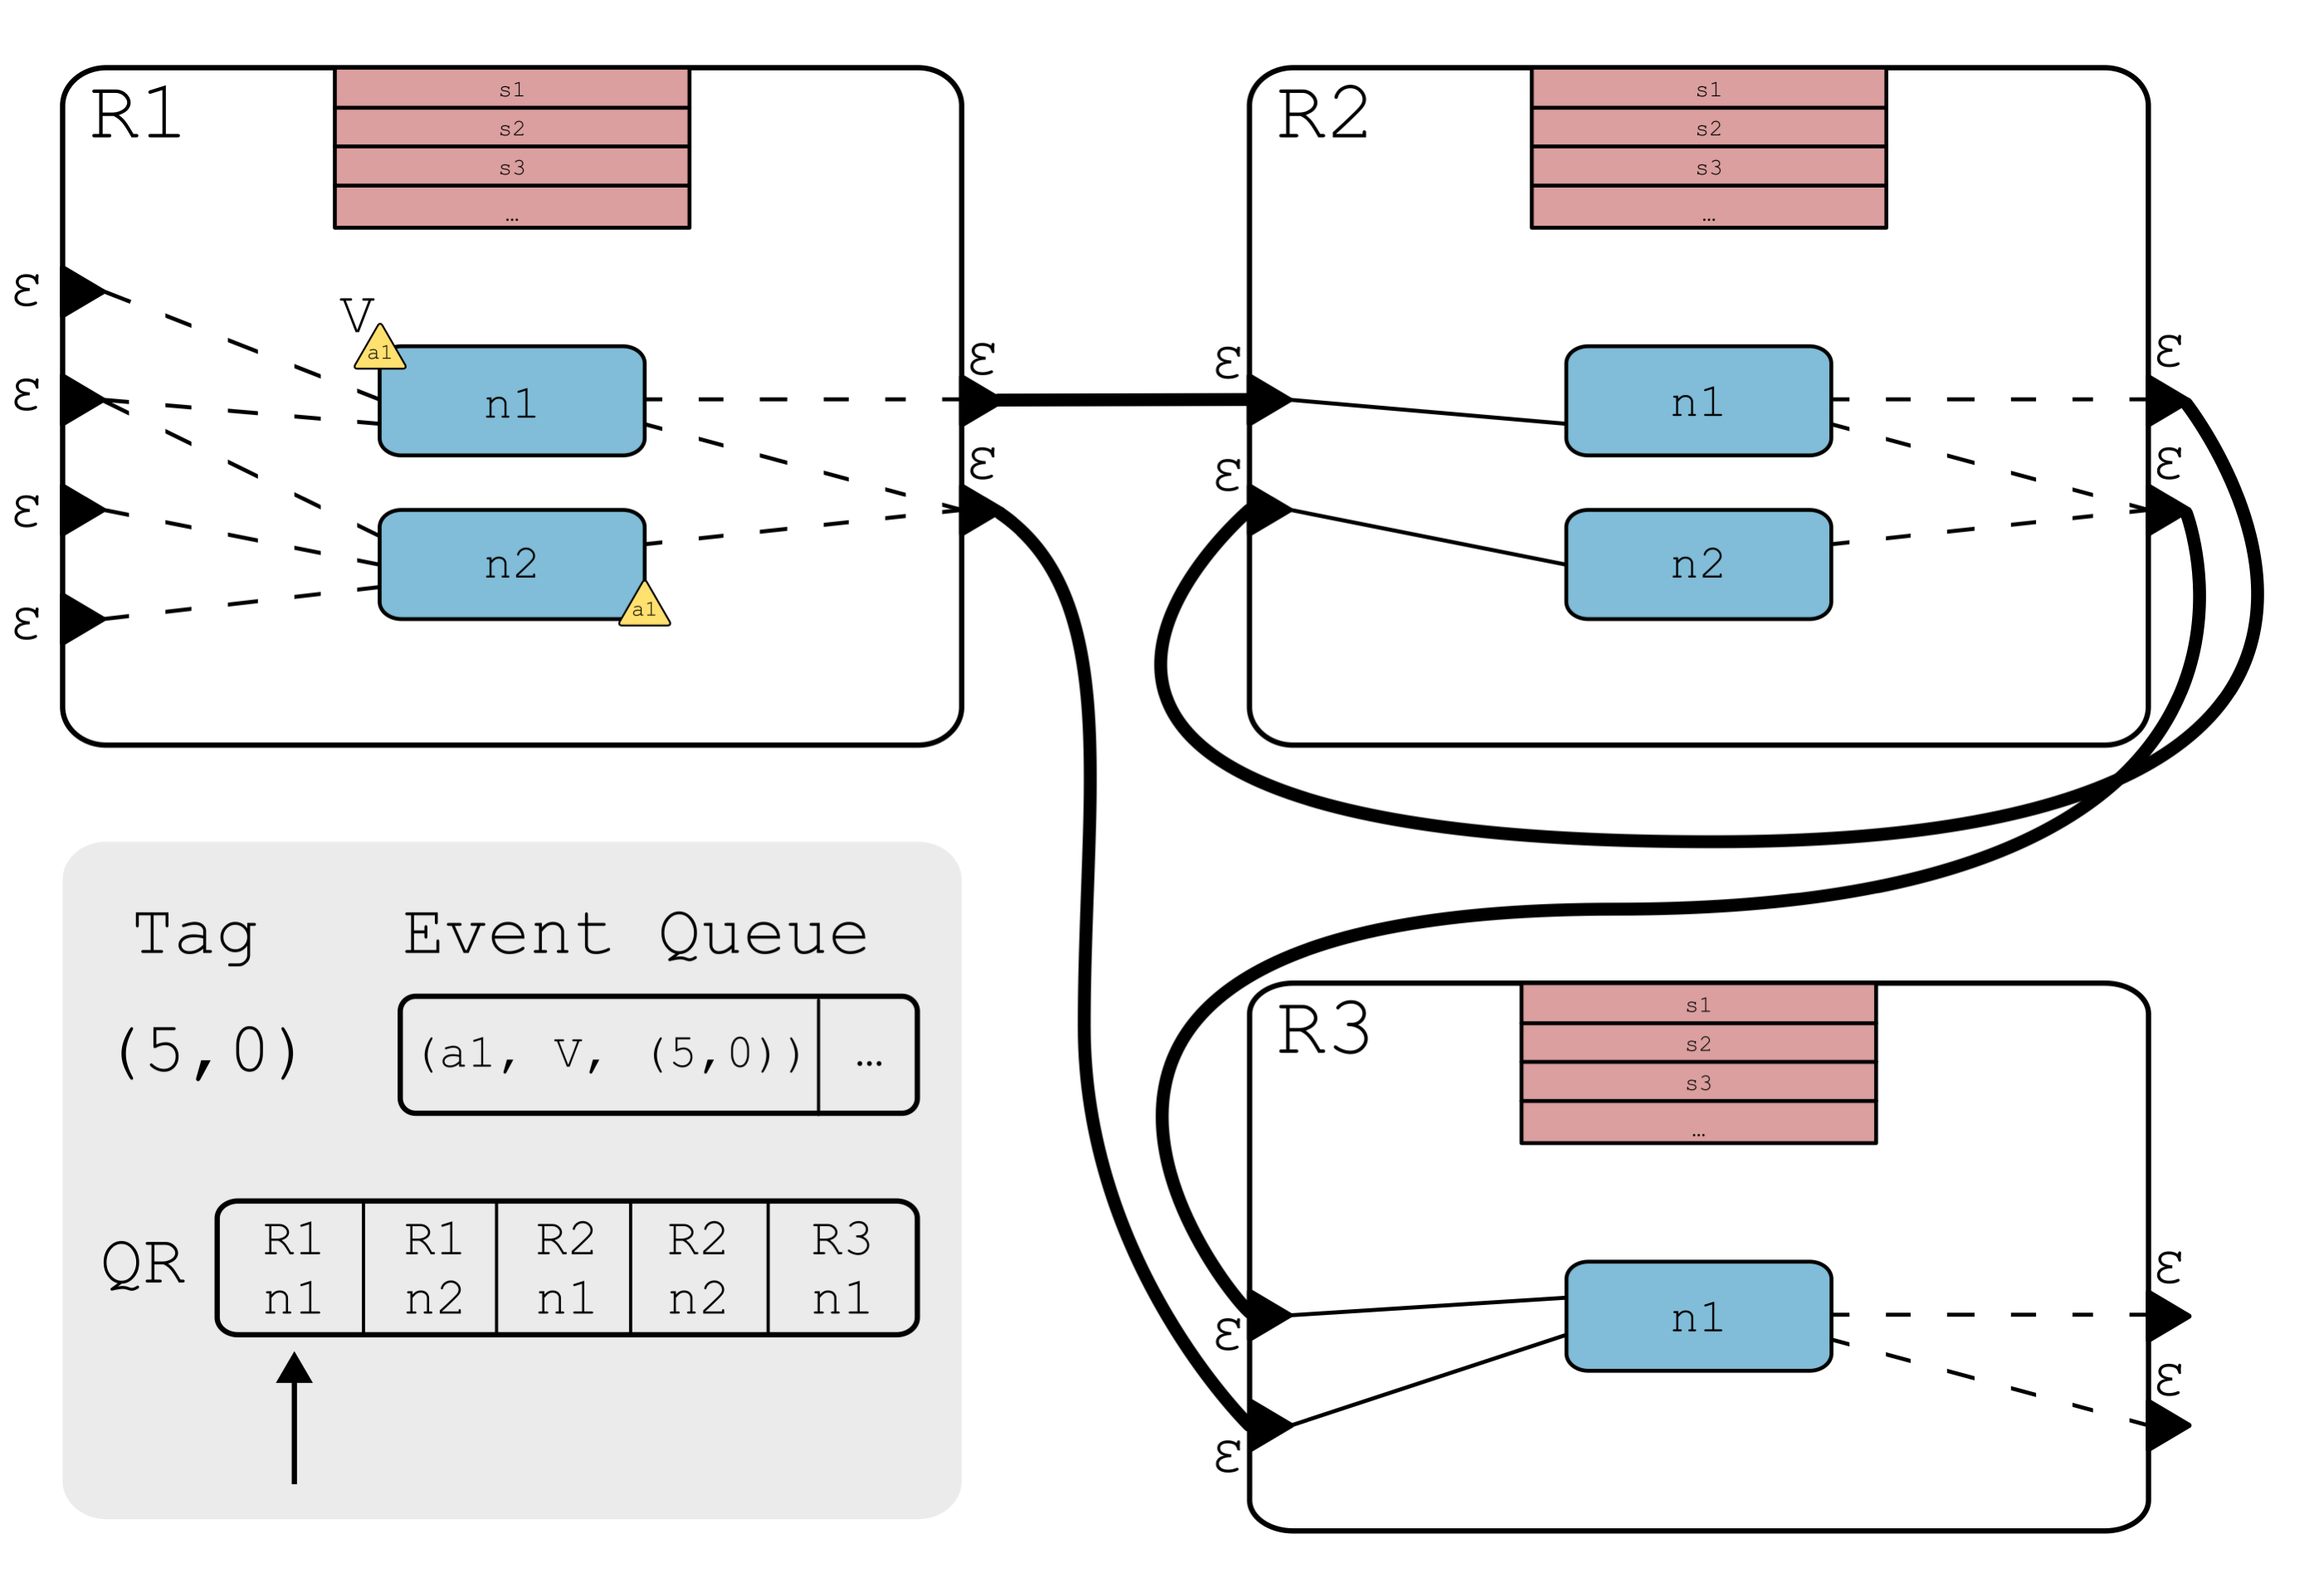
\includegraphics[width=\columnwidth]{exec-1}
\caption{Execution example --- right before $R1.n1$'s execution}
\label{fig:exec-1}
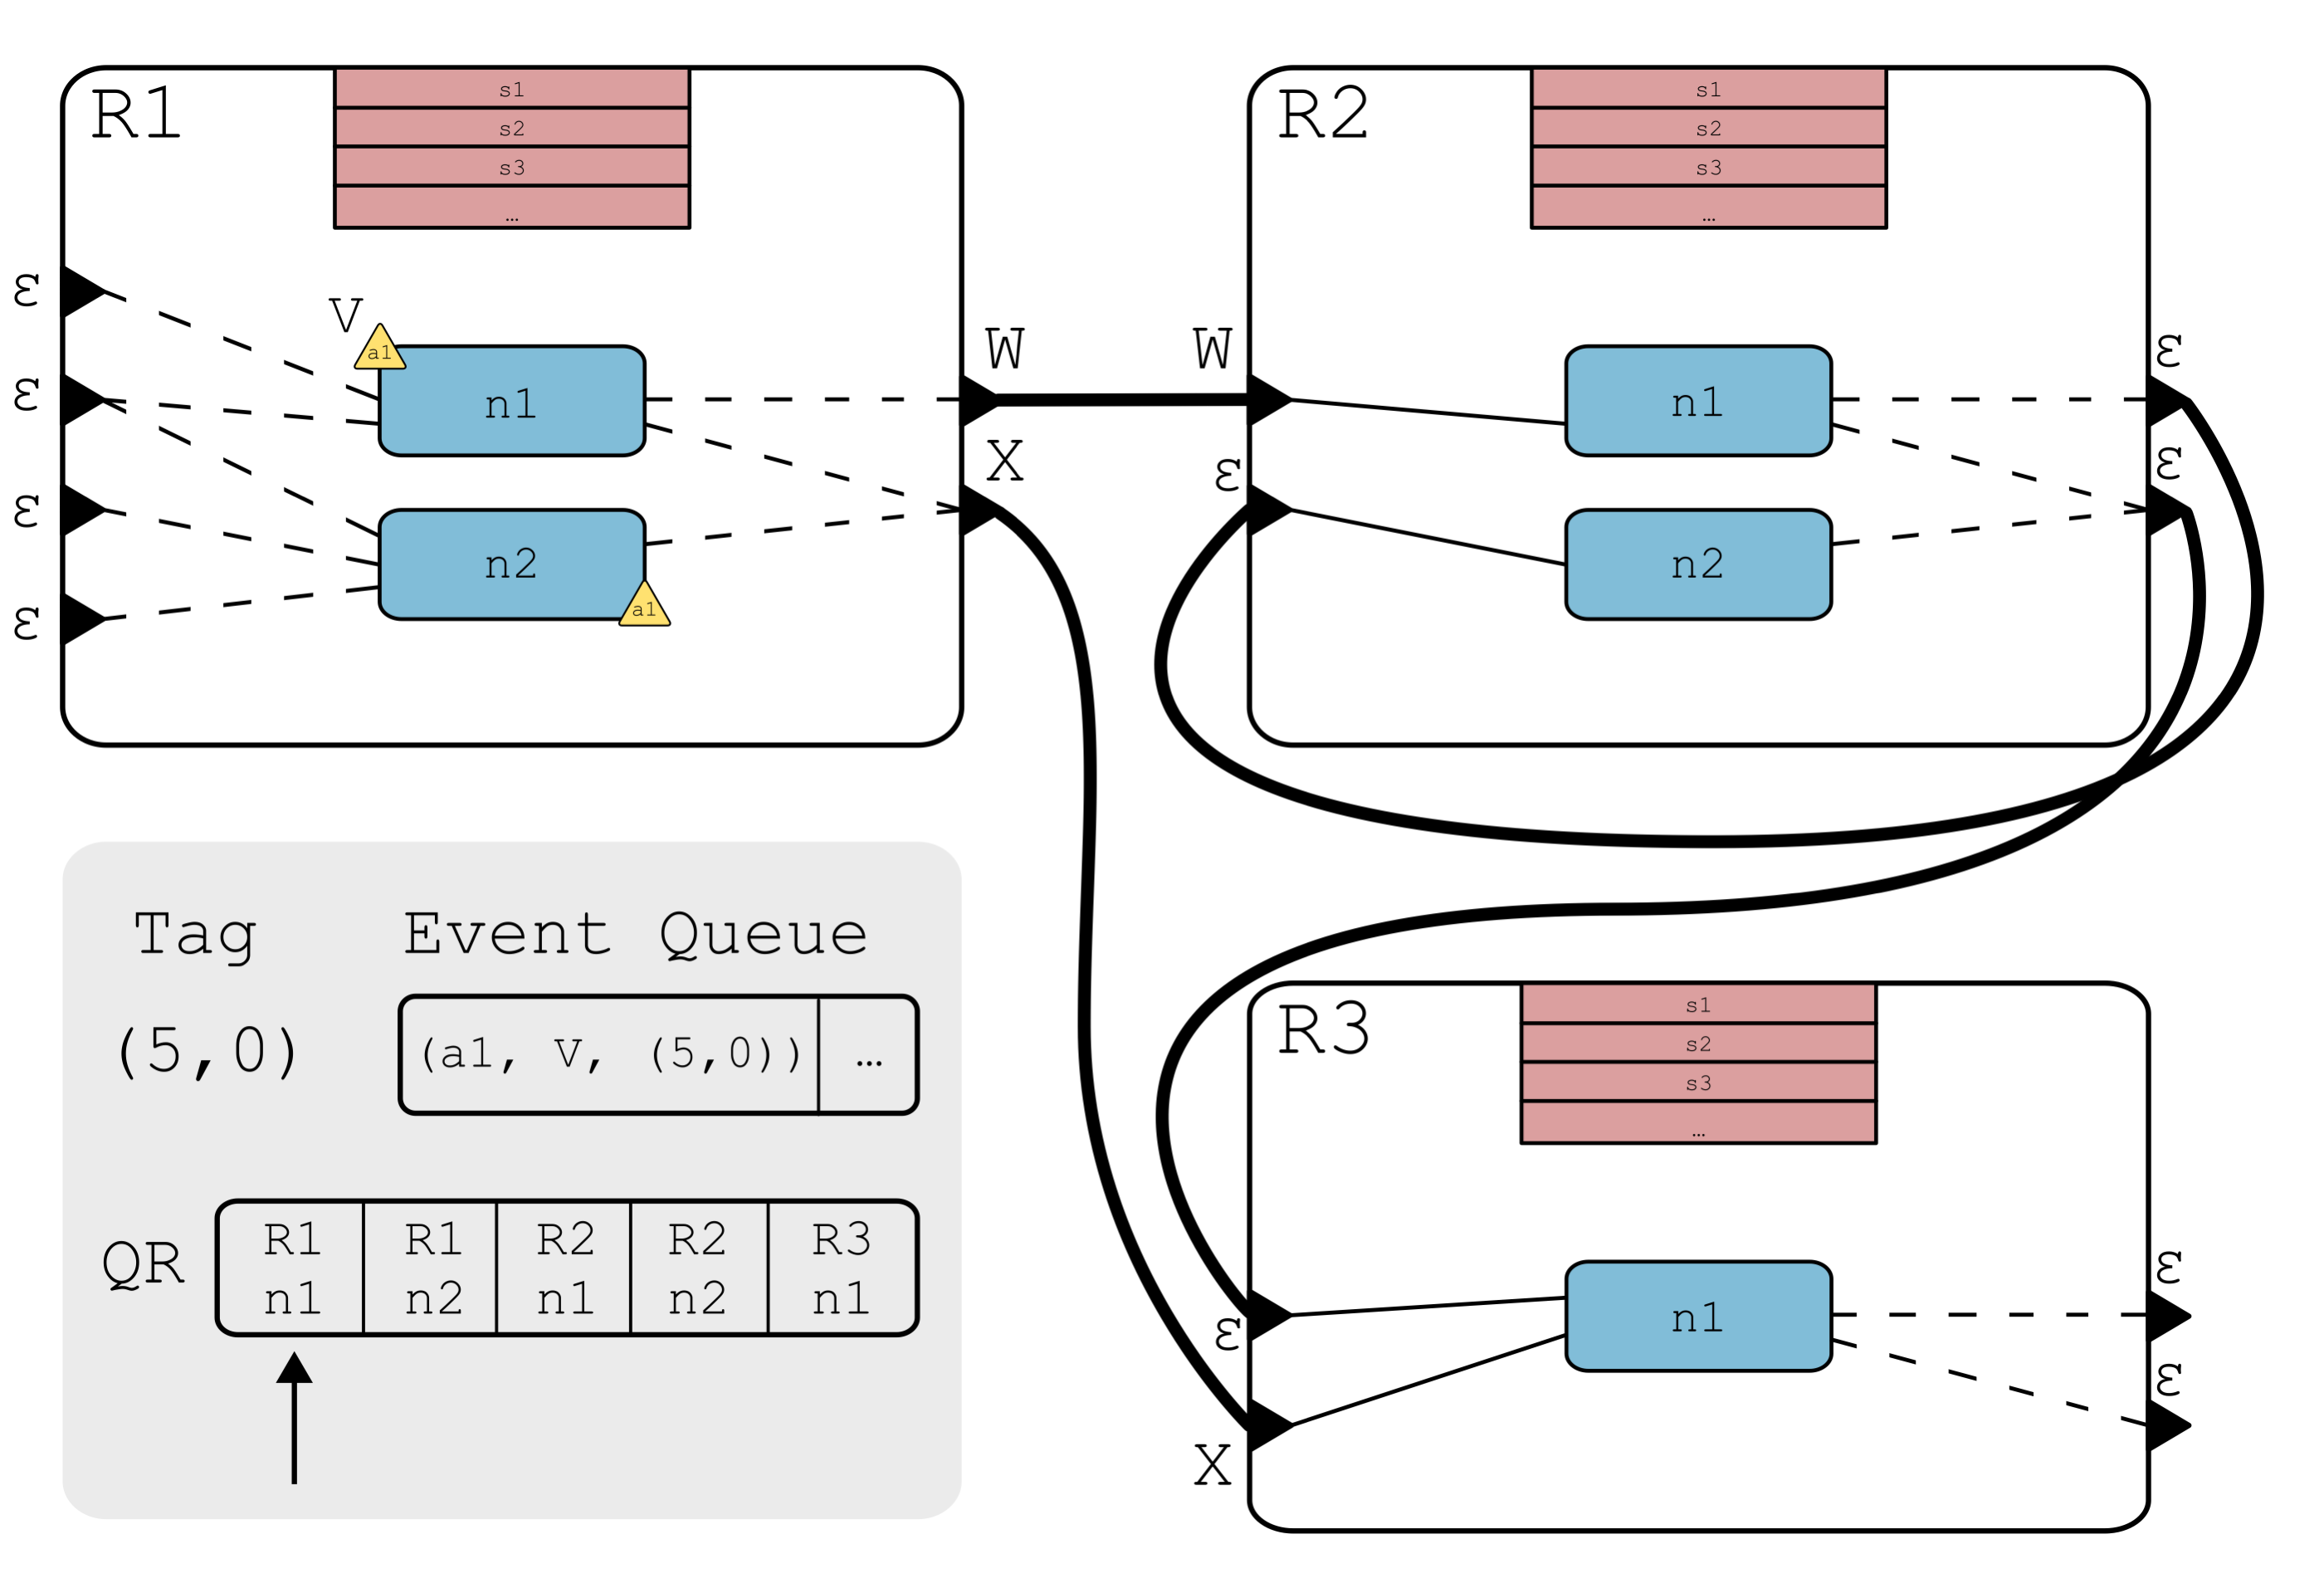
\includegraphics[width=\columnwidth]{exec-2}
\caption{Execution example --- after $R1.n1$'s values have been propagated}
\label{fig:exec-2}
\end{figure}

\begin{figure}[!htbp]
\centering
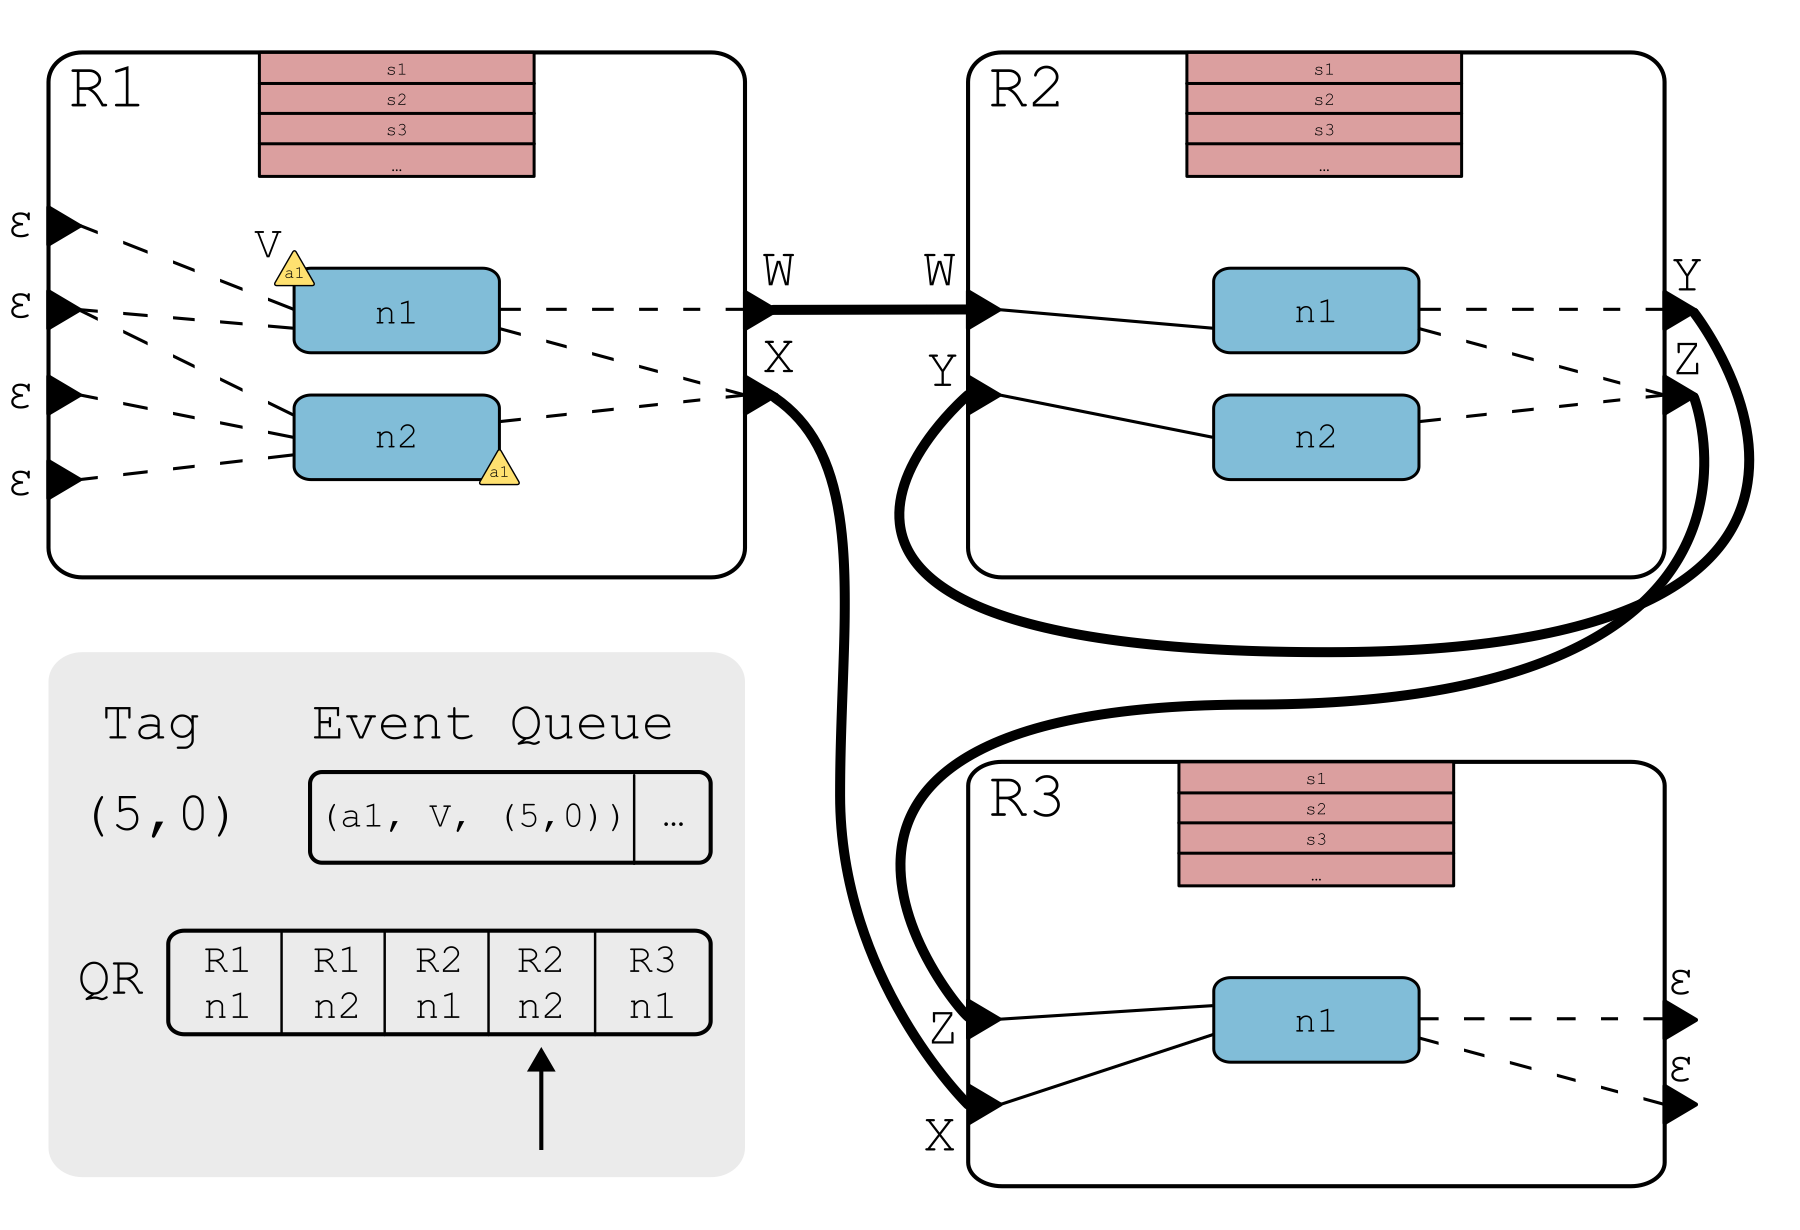
\includegraphics[width=\columnwidth]{exec-3}
\caption{Execution example --- right before $R2.n2$'s execution}
\label{fig:exec-3}
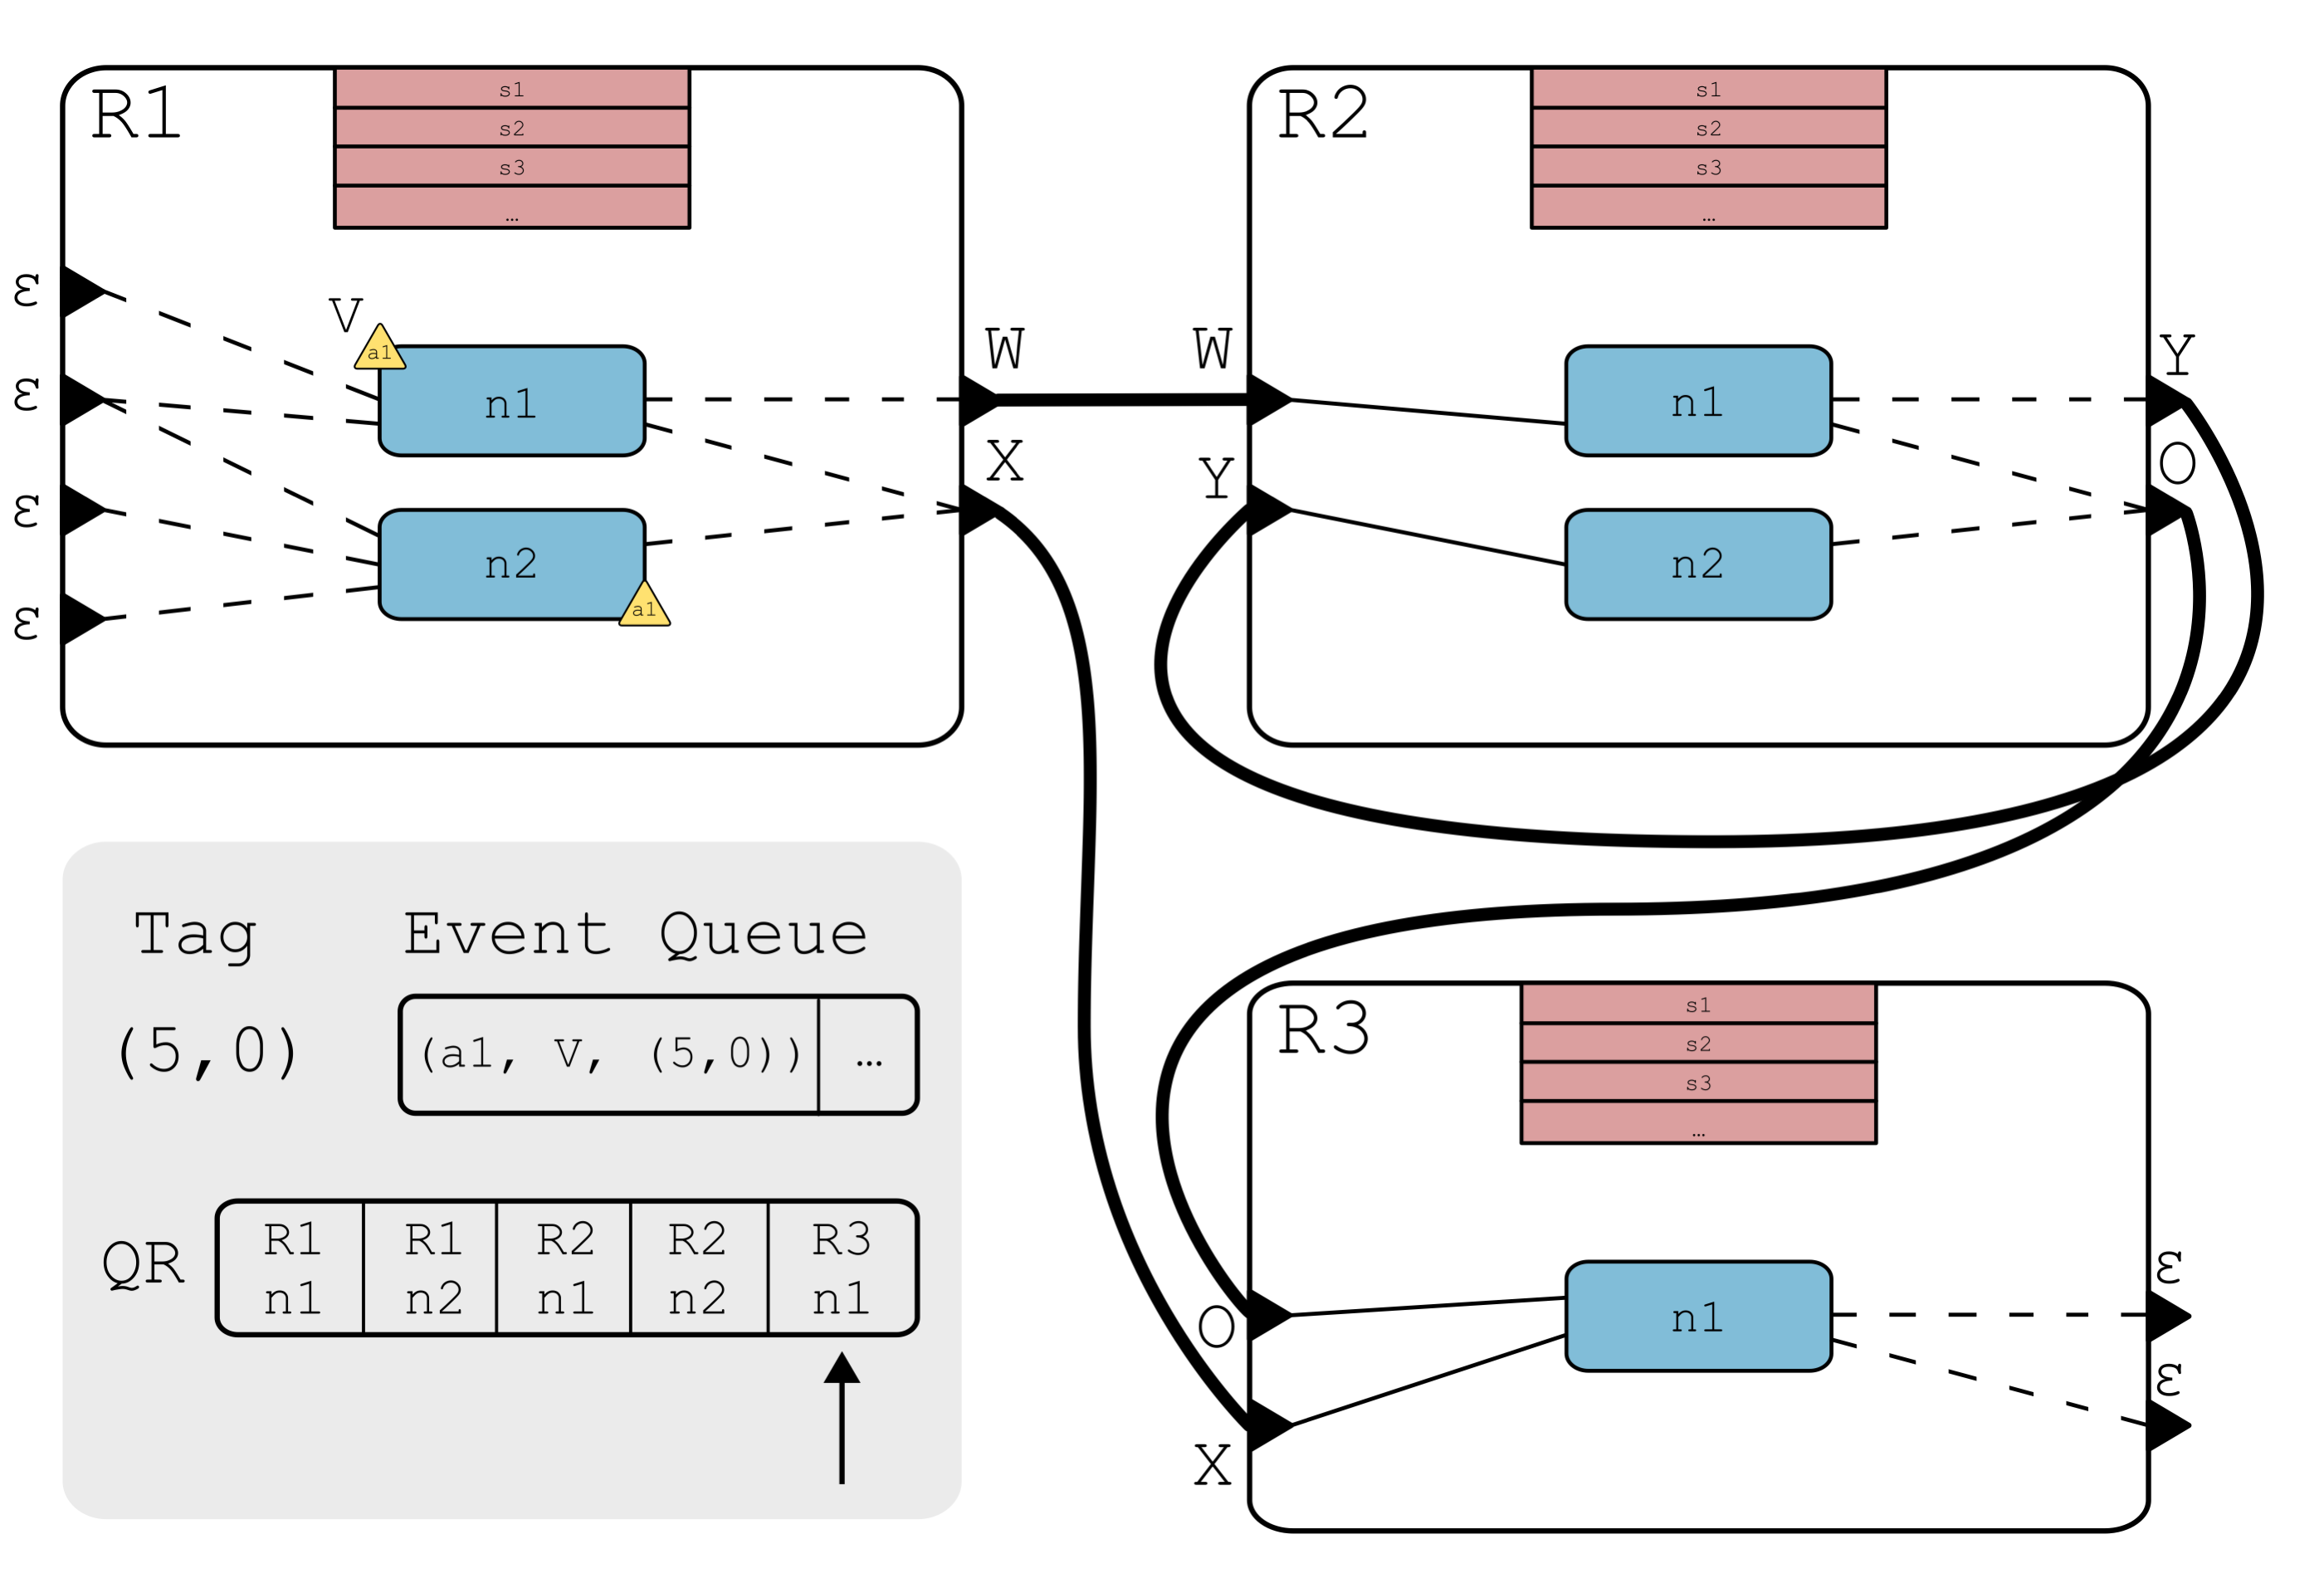
\includegraphics[width=\columnwidth]{exec-4}
\caption{Execution example --- right before $R3.n1$'s execution}
\label{fig:exec-4}
\end{figure}

\begin{figure}[!htbp]
\centering
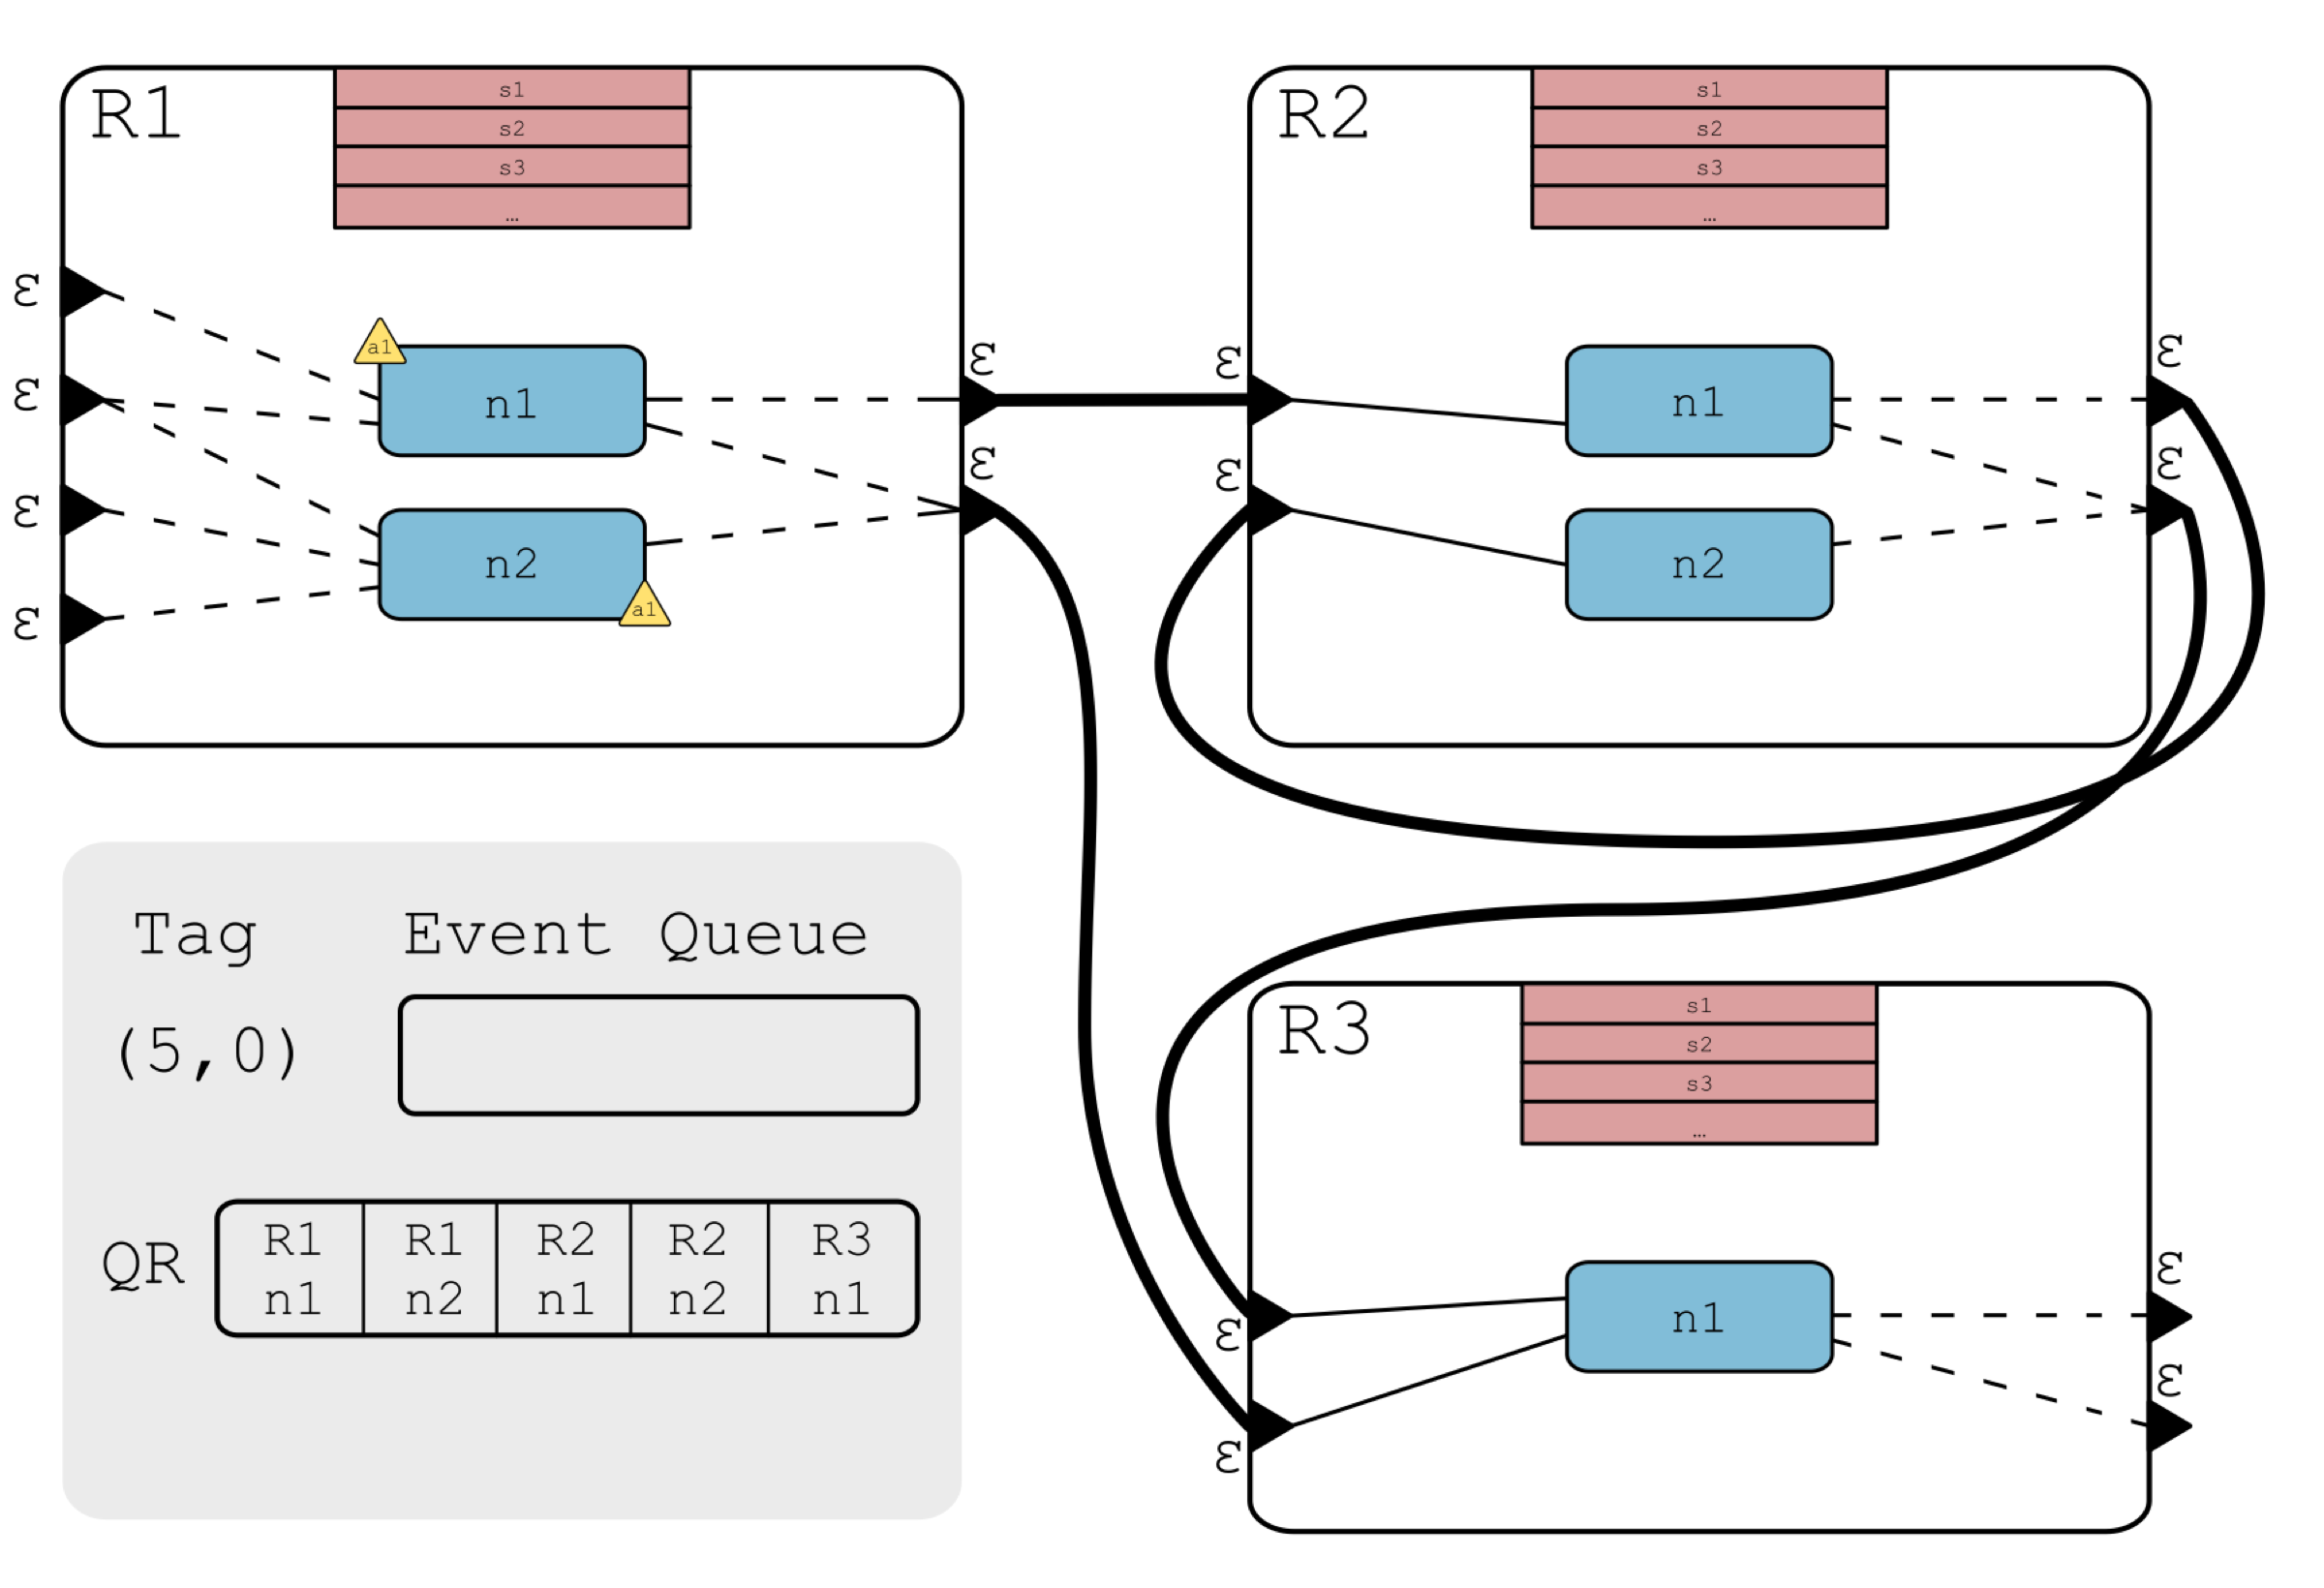
\includegraphics[width=\columnwidth]{exec-5}
\caption{Execution example --- end of execution}
\label{fig:exec-5}
\end{figure}

\break

\subsubsection{Inaccuracies}
\label{section:inaccuracies}

Despite our reduction from the full Reactor model, the formalization presented above has some issues that need to be addressed:

\begin{itemize}
    \item The definitions of reactors and reactions are circular.\footnote{
        In \cite{cyphy}, the circularity isn't as direct.
        There, the interdependency of definitions goes reactors $\to$ reactions $\to$ container function $\to$ reactors.
    }
    \item The concept of \emph{opaque} objects used for identifiers, values and reaction bodies is not well-defined. 
    A rigorous formalization will need to back this up with something concrete.
    \item The actual ``position'' of values ($\in \mathfrak{V}$) is undefined.
    That is, there exists no map from identifiers to values.
    It is therefore impossible to obtain the values of components like ports or state variables.
    This issue has been addressed in \cite{marten} by defining affected fields, like a reactor's ports, as Cartesian products of identifiers and values.
    \item The definition of a reaction's body $B$ has the aforementioned problem of being opaque.
    For \emph{this} object especially, the opaqueness hinders us from creating any rigorous definitions of computation in a reaction — and hence in the Simple Reactor model in general.
    For example, it is not clear how reactions access the values associated with actions/events.  
    \item The definition of a reactor's reactions $\mathcal{N}$ as a \emph{set} disallows multiple identical reactions from living in the same reactor.
    Though this is not a problem from a mathematical standpoint, we consider it to be undesirable.
    As an example, consider Figure \ref{fig:unique-rcn}.
    Let the reactions' names ($1$, $2$, $3$) also be their priorities.
    Reactions $1$ and $3$ have the same dependencies, antidependencies, triggers and schedulable actions (none).
    If we also assume their bodies to be equal, the reactions are identical.
    The only differentiating factor are their priorities.
    As a reactor's set of reactions does not include the priorities, reactions $1$ and $3$ would collapse into a single element.
    Thus, our current model does not allow us to create the depicted reactor.
\end{itemize}

\begin{figure}[!h]
\centering
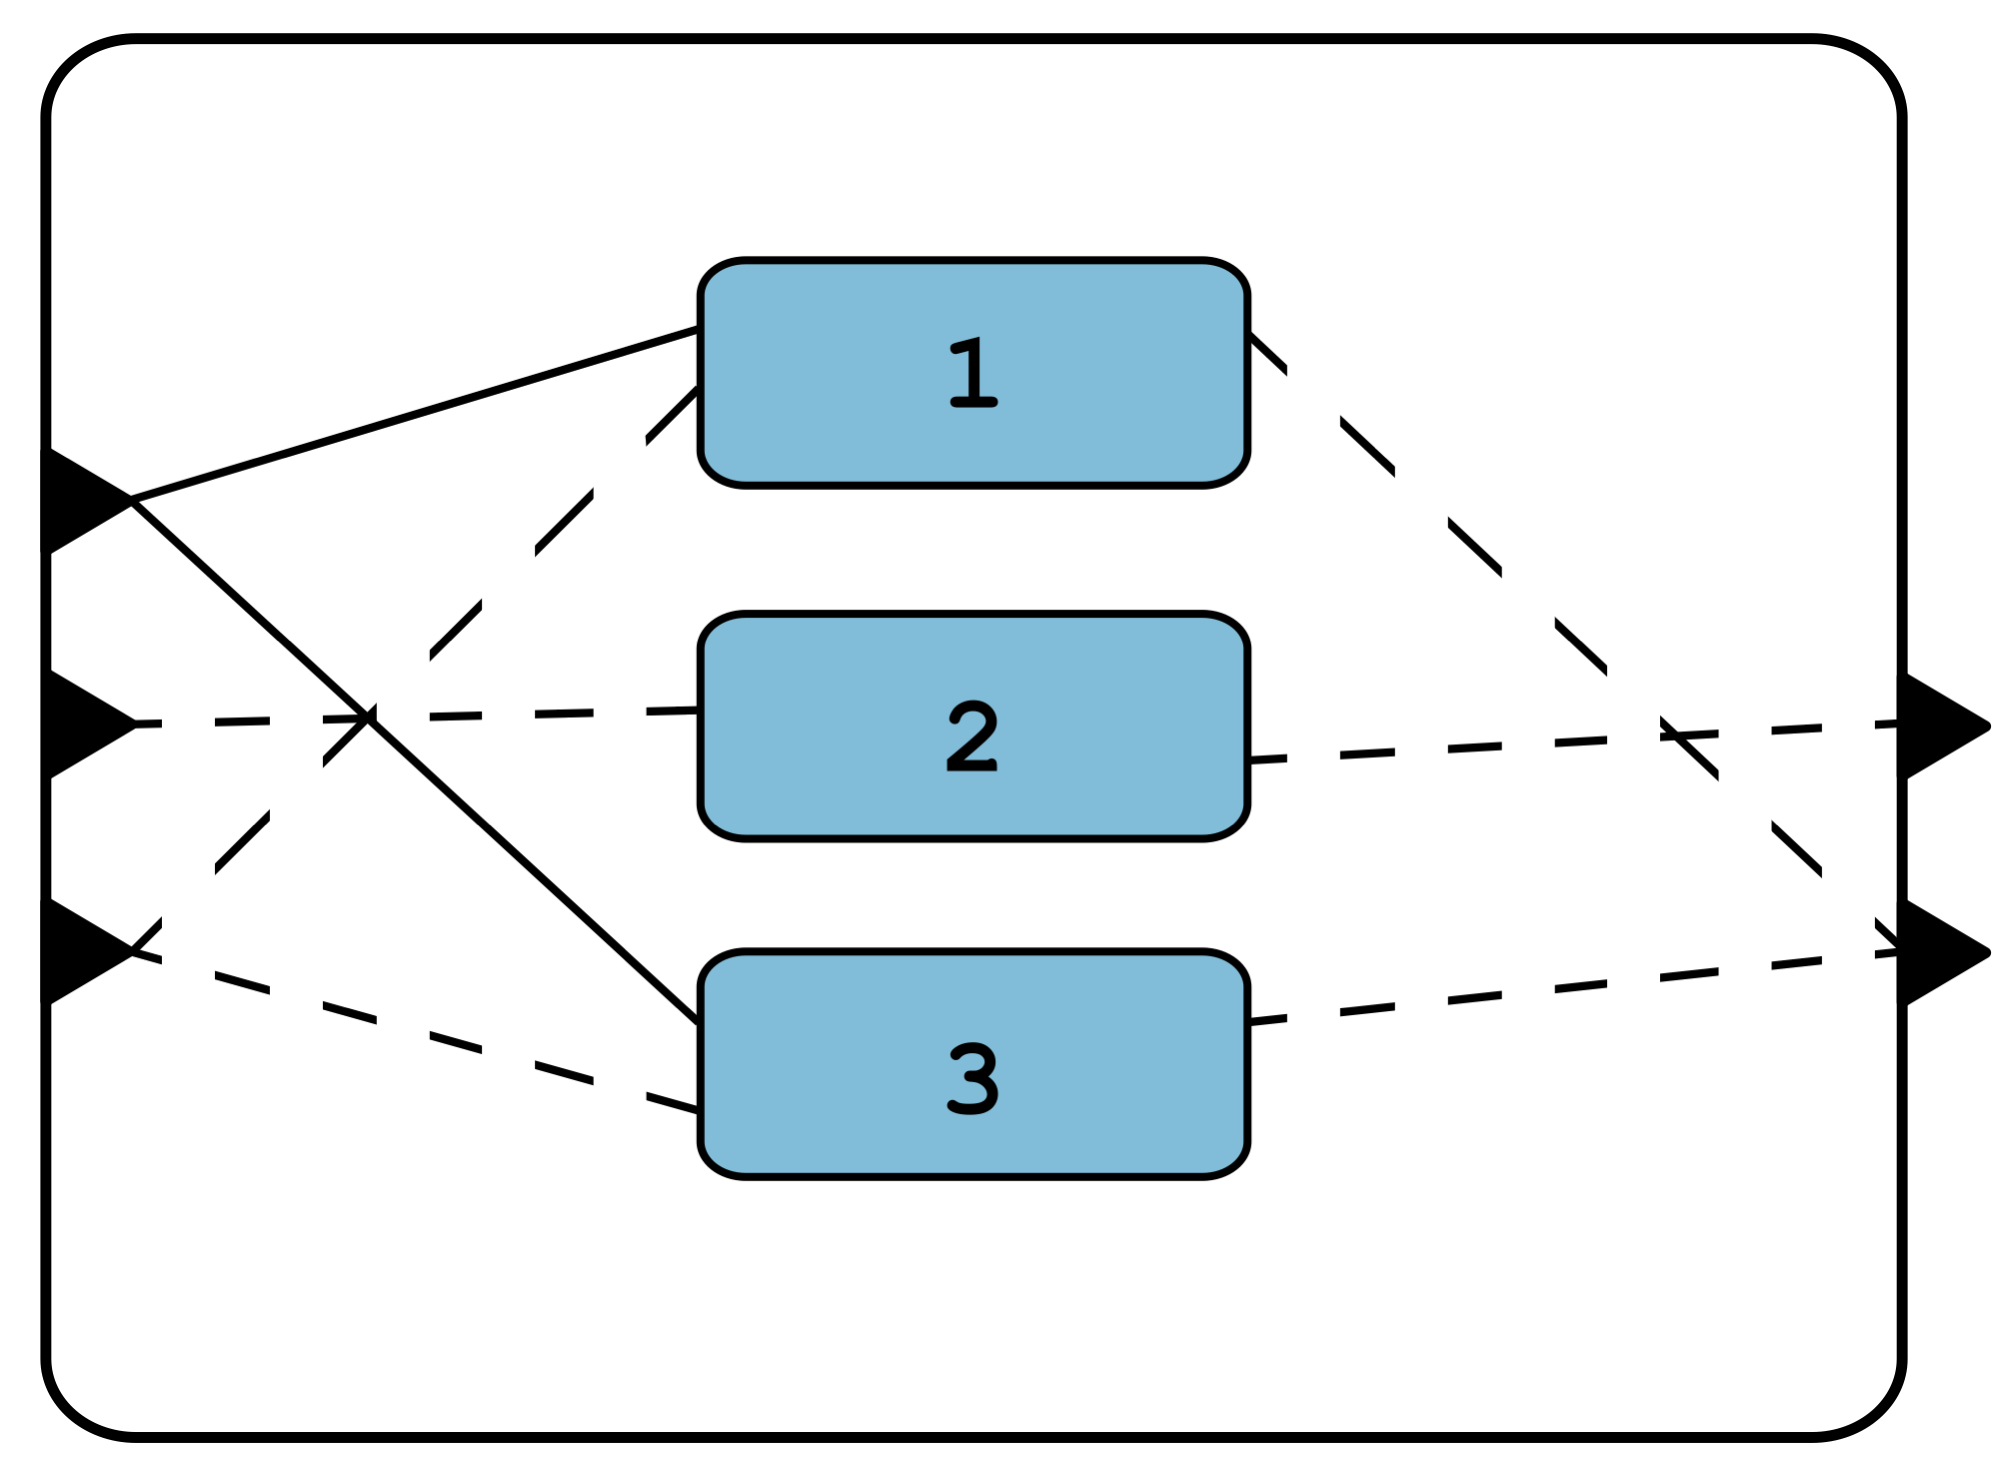
\includegraphics[width=0.4\columnwidth]{unique-rcn}
\caption{Example of identical reactions in the same reactor}
\label{fig:unique-rcn}
\end{figure}

\paragraph{Garbage In, Garbage Out:} 
We would like to emphasize here that the following aspect of the model is \emph{not} an issue:
we define no restrictions on the sets of identifiers in a reactor.
That is, a reactor's input ports $I$, output ports $O$ and state variables $S$ can contain \emph{any} identifiers.
This could be considered an issue, as a reactor could contain an identifier $i$ with $i \in I$, $i \in O$ \emph{and} $i \in S$.
Instead, it is rather representative of an approach to formalization used throughout this thesis.
It can be summarized by a principle called ``Garbage In, Garbage Out'' (GIGO), by which we mean:
If one defines nonsensical objects, like a reactor where a single identifier is used for multiple components, then it should not be expected that it behaves sensibly. 
This approach has the benefit of allowing us to focus an object's definition on what we \emph{want} its properties to be, without having to be precise about the properties it should \emph{not} have.
Hence, the definitions above can be viewed as necessary but not sufficient for well-behaved reactors.
